\section{משוואת לפלס – הקדמה ומשפטי יחידות}

\subsection{רקע פיזיקלי ומשוואת לפלס}
משוואת לפלס (\LR{Laplace's Equation}) היא משוואה דיפרנציאלית חלקית המתארת תופעות פיזיקליות רבות במצב עמיד (\LR{Steady State}). באופן היסטורי, המשוואה נובעת מאלקטרוסטטיקה. חוק גאוס הדיפרנציאלי קובע כי:
\[
\vec{\nabla} \cdot \vec{E} = \frac{\rho}{\epsilon_0}
\]
כאשר נציב את הקשר לפוטנציאל החשמלי, $\vec{E} = -\vec{\nabla} \phi$, נקבל את משוואת פואסון (\LR{Poisson's Equation}):
\[
\nabla^2 \phi = -\frac{\rho}{\epsilon_0}
\]
באזורים בהם אין צפיפות מטען ($\rho=0$), אנו מקבלים את משוואת לפלס:
\begin{definitionbox}{משוואת לפלס}
\[
\nabla^2 u(\vec{r}) = 0
\]
כאשר $u$ היא הפונקציה הנעלמה (פוטנציאל חשמלי, טמפרטורה, וכו'). פתרונות של משוואת לפלס נקראים \textbf{פונקציות הרמוניות} (\LR{Harmonic Functions}).
\end{definitionbox}

המשוואה מופיעה בהקשרים פיזיקליים נוספים:
\begin{enumerate}
    \item דיפוזיה במצב עמיד משוואת הדיפוזיה היא $\frac{\partial u}{\partial t} = D \nabla^2 u$. במצב עמיד ($\frac{\partial u}{\partial t} = 0$), התפלגות הטמפרטורה (או הריכוז) מקיימת $\nabla^2 u = 0$.
    \item הידרודינמיקה זרימה פוטנציאלית של נוזל בלתי-דחיס וחסר צמיגות.
\end{enumerate}

\subsection{הלפלסיאן בקואורדינטות שונות}
במשוואת לפלס, בחירת מערכת הקואורדינטות היא קריטית ותלויה בסימטריה של הבעיה ושפתה.

\begin{resultbox}{אופרטור הלפלסיאן ($\nabla^2$) בקואורדינטות נפוצות}
\textbf{קואורדינטות קרטזיות $(x,y,z)$:}
\[
\nabla^2 u = \frac{\partial^2 u}{\partial x^2} + \frac{\partial^2 u}{\partial y^2} + \frac{\partial^2 u}{\partial z^2}
\]
\textbf{קואורדינטות גליליות $(r,\phi,z)$:}
\[
\nabla^2 u = \frac{1}{r} \frac{\partial}{\partial r} \left( r \frac{\partial u}{\partial r} \right) + \frac{1}{r^2} \frac{\partial^2 u}{\partial \phi^2} + \frac{\partial^2 u}{\partial z^2}
\]
\textbf{קואורדינטות כדוריות $(r,\theta,\varphi)$:}
\[
\nabla^2 u = \frac{1}{r^2} \frac{\partial}{\partial r} \left( r^2 \frac{\partial u}{\partial r} \right) + \frac{1}{r^2 \sin \theta} \frac{\partial}{\partial \theta} \left( \sin \theta \frac{\partial u}{\partial \theta} \right) + \frac{1}{r^2 \sin^2 \theta} \frac{\partial^2 u}{\partial \varphi^2}
\]
\end{resultbox}

\section{פתרונות חד-ממדיים וסימטריה}
במקרים בהם קיימת סימטריה גבוהה, ניתן להניח שהפוטנציאל תלוי בקואורדינטה אחת בלבד. במקרים אלו, המד"ח הופכת למד"ר פשוטה. נבחן שלושה מקרים קלאסיים.

\subsection{קואורדינטות קרטזיות – קבל לוחות}
נתונים שני לוחות אינסופיים (או שמימדיהם גדולים מאוד ביחס למרחק ביניהם $L$) במישורים $x=0$ ו-$x=L$. הפוטנציאל על הלוחות הוא $u(0)=u_L$ ו-$u(L)=u_R$.
בשל הסימטריה (אין תלות ב-$y$ או ב-$z$), נניח $u=u(x)$. המשוואה היא $\frac{d^2 u}{dx^2} = 0$.
\begin{center}
    
\begin{tikzpicture}
\draw[thick] (0,0) -- (0,3) node[above] {$u_L$};
\draw[thick] (4,0) -- (4,3) node[above] {$u_R$};
\draw[<->] (0,1.5) -- (4,1.5) node[midway, above] {$L$};
\draw[->] (0,0) -- (5,0) node[right] {$x$};
\draw[->] (0,0) -- (0,3.5) node[above] {$y/z$};
\end{tikzpicture}
\end{center}

\begin{examplebox}{פתרון לקבל לוחות}
פתרון המשוואה $u''(x)=0$ הוא פונקציה ליניארית:
\[ u(x) = Ax + B \]
לאחר הצבת תנאי השפה:
\[ u(x) = (u_R - u_L)\frac{x}{L} + u_L \]
זהו הפתרון היחיד (כפי שנוכיח בהמשך). במציאות, עבור לוחות סופיים, בקצוות יהיו תיקונים \LR{("edge effects ")}, אך בקירוב של לוחות אינסופיים הפוטנציאל תלוי ב-$x$ בלבד.
\end{examplebox}

\subsection{קואורדינטות גליליות – קבל גלילי}
נתון גליל אינסופי בציר $z$. נתונים שני משטחים גליליים ברדיוסים $r=a$ ו-$r=b$ עם פוטנציאלים $u_a$ ו-$u_b$ בהתאמה.
בשל הסימטריה (אינווריאנטיות לסיבוב ב-$\phi$ ולהזזה ב-$z$), הפוטנציאל הוא $u=u(r)$.
המשוואה:
\[ \frac{1}{r} \frac{d}{dr} \left( r \frac{du}{dr} \right) = 0 \]

\begin{examplebox}{פתרון לקבל גלילי}
נכפיל ב-$r$ ונבצע אינטגרציה:
\[ r \frac{du}{dr} = C_1 \implies \frac{du}{dr} = \frac{C_1}{r} \]
אינטגרציה נוספת נותנת:
\[ u(r) = C_1 \ln r + C_2 \]
נציב תנאי שפה $u(a)=u_a, u(b)=u_b$ ומקבלים:
\[ u(r) = u_a + (u_b - u_a) \frac{\ln(r/a)}{\ln(b/a)} \]
\textbf{הערה פיזיקלית:} אם התחום כולל את הראשית ($a=0$), הפתרון הלוגריתמי מתבדר. אם אין מטען קווי בראשית ("Line Charge"), עלינו לדרוש $C_1=0$ כדי שהפוטנציאל יהיה חסום, ונקבל פוטנציאל קבוע.
\end{examplebox}

\subsection{קואורדינטות כדוריות – קבל כדורי}
נתונות שתי קליפות כדוריות ברדיוסים $a$ ו-$b$ עם פוטנציאלים קבועים. מטעמי סימטריה כדורית, $u=u(r)$.
המשוואה:
\[ \frac{1}{r^2} \frac{d}{dr} \left( r^2 \frac{du}{dr} \right) = 0 \]

\begin{examplebox}{פתרון לקבל כדורי}
נבצע אינטגרציה פעמיים:
\[ r^2 \frac{du}{dr} = C_1 \implies \frac{du}{dr} = \frac{C_1}{r^2} \]
\[ u(r) = -\frac{C_1}{r} + C_2 \]
הפתרון הוא מהצורה $u(r) = \frac{A}{r} + B$.
עבור תנאי שפה כלליים $u(a)=u_a$ ו-$u(b)=u_b$:
\[ u(r) = u_a + (u_b - u_a) \frac{\frac{1}{r} - \frac{1}{a}}{\frac{1}{b} - \frac{1}{a}} \]
אם נדרוש $u(b) \to 0$ כאשר $b \to \infty$ ונתון מטען $Q$ במרכז, נקבל את הפוטנציאל המוכר של מטען נקודתי: $u(r) \propto \frac{Q}{r}$.
\end{examplebox}

\section{משפטי קיום ויחידות}

התכונה החשובה ביותר של משוואת לפלס היא היחידות: אם מצאנו (אפילו בניחוש) פונקציה המקיימת את המשוואה ואת תנאי השפה, זוהי הפונקציה היחידה.

\subsection{סוגי תנאי שפה}
נתון נפח $V$ הכלוא על ידי משטח $S$.
\begin{enumerate}
    \item תנאי דיריכלה (\LR{Dirichlet}) הערך של הפונקציה $u$ נתון על השפה $S$.
    \[ u|_S = f(\vec{r}) \]
    \item תנאי נוימן (\LR{Neumann}) הנגזרת הנורמלית של הפונקציה נתונה על השפה $S$.
    \[ \frac{\partial u}{\partial n}\bigg|_S = \vec{\nabla} u \cdot \hat{n} = g(\vec{r}) \]
\end{enumerate}

\subsection{משפט היחידות הראשון (דיריכלה)}
\begin{theorembox}{משפט היחידות (תנאי שפה דיריכלה)}
אם $u_1$ ו-$u_2$ הם שני פתרונות של משוואת לפלס $\nabla^2 u = 0$ בנפח $V$, המקיימים את אותו תנאי שפה $u|_S = f$, אזי $u_1(\vec{r}) = u_2(\vec{r})$ לכל $\vec{r} \in V$.
\end{theorembox}

\textbf{הוכחה:}
נגדיר פונקציית הפרש $w = u_1 - u_2$. מכיוון שהלפלסיאן הוא אופרטור לינארי:
\[ \nabla^2 w = \nabla^2 u_1 - \nabla^2 u_2 = 0 \]
על השפה, $w|_S = u_1|_S - u_2|_S = f - f = 0$.
נשתמש בזהות וקטורית עבור הדיברגנץ של המכפלה $w \vec{\nabla} w$:
\[ \vec{\nabla} \cdot (w \vec{\nabla} w) = (\vec{\nabla} w)^2 + w \nabla^2 w \]
מכיוון ש-$\nabla^2 w = 0$, נקבל $\vec{\nabla} \cdot (w \vec{\nabla} w) = (\vec{\nabla} w)^2$.
נבצע אינטגרל נפחי ונשתמש במשפט הדיברגנץ (משפט גאוס):
\[ \iiint_V (\vec{\nabla} w)^2 dV = \iiint_V \vec{\nabla} \cdot (w \vec{\nabla} w) dV = \oiint_S (w \vec{\nabla} w) \cdot \hat{n} dS \]
באגף ימין, האינטגרל הוא על השפה $S$. מאחר ש-$w|_S = 0$, האינטגרל כולו מתאפס.
קיבלנו:
\[ \iiint_V |\vec{\nabla} w|^2 dV = 0 \]
מכיוון שהאינטגרנד $|\vec{\nabla} w|^2$ הוא אי-שלילי תמיד, האינטגרל יכול להתאפס רק אם האינטגרנד מתאפס זהותית בכל הנפח:
\[ \vec{\nabla} w = 0 \implies w = \text{const} \]
מכיוון שעל השפה $w=0$, הקבוע חייב להיות 0. לכן $w=0$ בכל הנפח, ו-$u_1 = u_2$. $\blacksquare$

\subsection{משפט היחידות השני (נוימן)}
עבור תנאי נוימן, $\frac{\partial u}{\partial n}|_S$ נתון. ההוכחה דומה, אך באינטגרל המשטחי:
\[ \oiint_S w (\vec{\nabla} w \cdot \hat{n}) dS = \oiint_S w \frac{\partial w}{\partial n} dS \]
כאן $\frac{\partial w}{\partial n} = \frac{\partial u_1}{\partial n} - \frac{\partial u_2}{\partial n} = g - g = 0$.
לכן שוב נקבל $\vec{\nabla} w = 0 \implies w = \text{const}$.
במקרה זה, איננו יכולים לקבוע שהקבוע הוא 0.
\begin{resultbox}{מסקנה}
עבור תנאי שפה נוימן, הפתרון למשוואת לפלס יחיד \textbf{עד כדי קבוע אדיטיבי}.
\end{resultbox}

\section{משוואת לפלס במישור חצי-אינסופי (2D)}

נבחן בעיה דו-ממדית בחצי המישור העליון $y > 0$.
\textbf{הבעיה:}
\begin{itemize}
    \item משוואה: $\nabla^2 u(x,y) = \frac{\partial^2 u}{\partial x^2} + \frac{\partial^2 u}{\partial y^2} = 0$ בתחום $-\infty < x < \infty, \quad y > 0$.
    \item תנאי שפה על השפה $y=0$: $u(x,0) = f(x)$.
    \item תנאי שפה באינסוף: $u \to 0$ כאשר $y \to \infty$ או $|x| \to \infty$.
\end{itemize}
\begin{center}
    
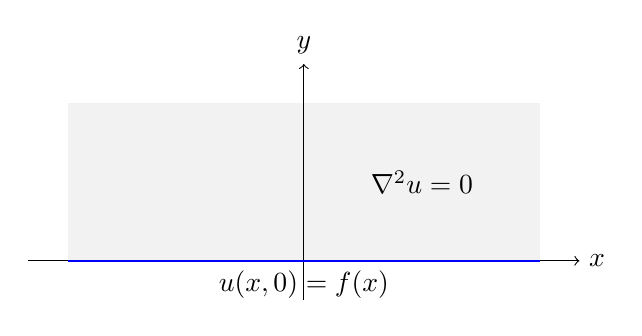
\begin{tikzpicture}
\fill[gray!10] (-3,0) rectangle (3,2);
\draw[->] (-3.5,0) -- (3.5,0) node[right] {$x$};
\draw[->] (0,-0.5) -- (0,2.5) node[above] {$y$};
\draw[thick, blue] (-3,0) -- (3,0) node[midway, below, black] {$u(x,0)=f(x)$};
\node at (1.5,1) {$\nabla^2 u = 0$};
\end{tikzpicture}
\end{center}

\subsection{פתרון באמצעות התמרת פורייה}
מכיוון שהתחום ב-$x$ הוא אינסופי ($-\infty < x < \infty$), נשתמש בהתמרת פורייה לפי $x$. נגדיר:
\[ \hat{u}(k,y) = \frac{1}{\sqrt{2\pi}} \int_{-\infty}^{\infty} u(x,y) e^{-ikx} dx \]
נבצע התמרה על משוואת לפלס:
\[ \mathcal{F} \left\{ \frac{\partial^2 u}{\partial x^2} \right\} + \mathcal{F} \left\{ \frac{\partial^2 u}{\partial y^2} \right\} = 0 \]
עבור הנגזרת ב-$x$, נקבל $(ik)^2 \hat{u} = -k^2 \hat{u}$. הנגזרת ב-$y$ אינה משתנה בהתמרה. נקבל מד"ר עבור $\hat{u}$ כפונקציה של $y$:
\[ \frac{d^2 \hat{u}}{dy^2} - k^2 \hat{u} = 0 \]
הפתרון הכללי הוא:
\[ \hat{u}(k,y) = A(k) e^{-|k|y} + B(k) e^{|k|y} \]
מכיוון שאנו דורשים שהפוטנציאל לא יתבדר ב-$y \to \infty$, נדרוש $B(k)=0$. לכן:
\[ \hat{u}(k,y) = A(k) e^{-|k|y} \]
ב-$y=0$, מתקיים $\hat{u}(k,0) = \hat{f}(k)$ (ההתמרה של תנאי השפה). לכן $A(k) = \hat{f}(k)$.
הפתרון במרחב התדר הוא:
\[ \hat{u}(k,y) = \hat{f}(k) e^{-|k|y} \]

\subsection{פונקציית גרין והחזרה למרחב המקום}
לפי משפט הקונבולוציה (Convolution), מכפלה במרחב התדר היא קונבולוציה במרחב המקום.
\[ u(x,y) = \frac{1}{\sqrt{2\pi}} \int_{-\infty}^{\infty} f(\xi) g(x-\xi, y) d\xi \]
כאשר $g(x,y)$ היא ההתמרה ההפוכה של הגורם $e^{-|k|y}$.
נחשב את ההתמרה ההפוכה של הגרעין $e^{-|k|y}$:
\[ K(x,y) = \frac{1}{\sqrt{2\pi}} \mathcal{F}^{-1} \{ e^{-|k|y} \} = \frac{1}{2\pi} \int_{-\infty}^{\infty} e^{-|k|y} e^{ikx} dk \]
האינטגרנד זוגי ב-$k$ (החלק המדומה $i\sin(kx)$ הוא אי-זוגי ומתאפס), לכן נחשב:
\[ K(x,y) = \frac{1}{\pi} \int_{0}^{\infty} e^{-ky} \cos(kx) dk \]
זהו אינטגרל סטנדרטי (ניתן לפתרון באמצעות אינטגרציה בחלקים פעמיים או שימוש בפונקציות מרוכבות). התוצאה היא:
\[ \int_{0}^{\infty} e^{-ky} \cos(kx) dk = \frac{y}{x^2 + y^2} \]
לכן, הגרעין (פונקציית גרין לבעיית חצי המישור) הוא:
\[ \frac{y}{\pi(x^2 + y^2)} \]
כאשר מבצעים את הקונבולוציה $u = f * K$, מקבלים את נוסחת האינטגרל של פואסון:

\begin{resultbox}{פתרון לחצי מישור עליון}
\[ u(x,y) = \frac{y}{\pi} \int_{-\infty}^{\infty} \frac{f(\xi)}{(x-\xi)^2 + y^2} d\xi \]
\end{resultbox}

\begin{notebox}{משמעות פיזיקלית והשוואה לדיפוזיה}
\begin{itemize}
    \item פונקציית גרין זו דועכת כמו $\frac{1}{x^2}$ (או פרופורציונלית ל-$1/r^2$ במישור). זוהי דעיכה "ארוכת טווח", הנובעת מאופי הכוחות החשמליים (כוחות ארוכי טווח).
    \item לשם השוואה, במשוואת הדיפוזיה קיבלנו גרעין גאוסיאני $e^{-x^2/4Dt}$, המייצג דעיכה מהירה מאוד. הסיבה היא שמנגנון הדיפוזיה מבוסס על התנגשויות אקראיות קצרות טווח.
\end{itemize}
\end{notebox}

\subsection{דוגמה: פוטנציאל קבוע על השפה}
נניח $f(x) = V_0$ (קבוע).
נציב בנוסחה:
\[ u(x,y) = \frac{V_0 y}{\pi} \int_{-\infty}^{\infty} \frac{d\xi}{(x-\xi)^2 + y^2} \]
נבצע החלפת משתנים $t = \frac{\xi - x}{y}$, אזי $d\xi = y dt$:
\[ u(x,y) = \frac{V_0}{\pi} \int_{-\infty}^{\infty} \frac{1}{t^2 + 1} dt = \frac{V_0}{\pi} [\arctan(t)]_{-\infty}^{\infty} \]
\[ u(x,y) = \frac{V_0}{\pi} \left( \frac{\pi}{2} - \left(-\frac{\pi}{2}\right) \right) = V_0 \]
קיבלנו ש-$u(x,y) = V_0$ בכל המרחב, תוצאה הצפויה ממשפט היחידות (פונקציה קבועה מקיימת את משוואת לפלס ואת תנאי השפה).